\section{A Check Outside Biomedicine}
\label{sec:cs}

Everything above was developed and measured on biomedical articles. The tool is meant for other fields too,
so we ran the released model on a computer-science paper: \emph{Probabilistic Data-Driven Sampling via
Multi-Criteria Importance Analysis} (Biswas et al., IEEE TVCG), a 17-page visualisation paper with 21 figures
and 423 body sentences. It differs from the training papers in almost every respect: field, length, number of
figures, and the kind of figure (scientific renderings and plots).

\paragraph{Set-up.} The paper was parsed from its PDF by the tool's own parser. No human gold exists for it. As a
stand-in, two large language models (Claude and Gemini) each labelled the sentences associated with every
figure. Both received the same numbered sentence list that the methods see, so that labels and predictions
refer to identical sentences, and a sentence counts as ``gold'' when the two labellers agree on it. We then
scored three systems against this reference: Paragraph, \bof{}, and the early-stopped span tagger SPAN\_ES.
SPAN\_ES used the decision rule fixed on the 15 training papers (raw logit $\ge 1.7$, citing sentences always
included); nothing was tuned on this paper. The model ran on a laptop and scored all $21\times423=8{,}883$ (figure, sentence) pairs in about three
minutes; a GPU would be faster. Figure~\ref{fig:cs} shows the
run and Table~\ref{tab:cs} the numbers.

\begin{figure}[h]
\centering
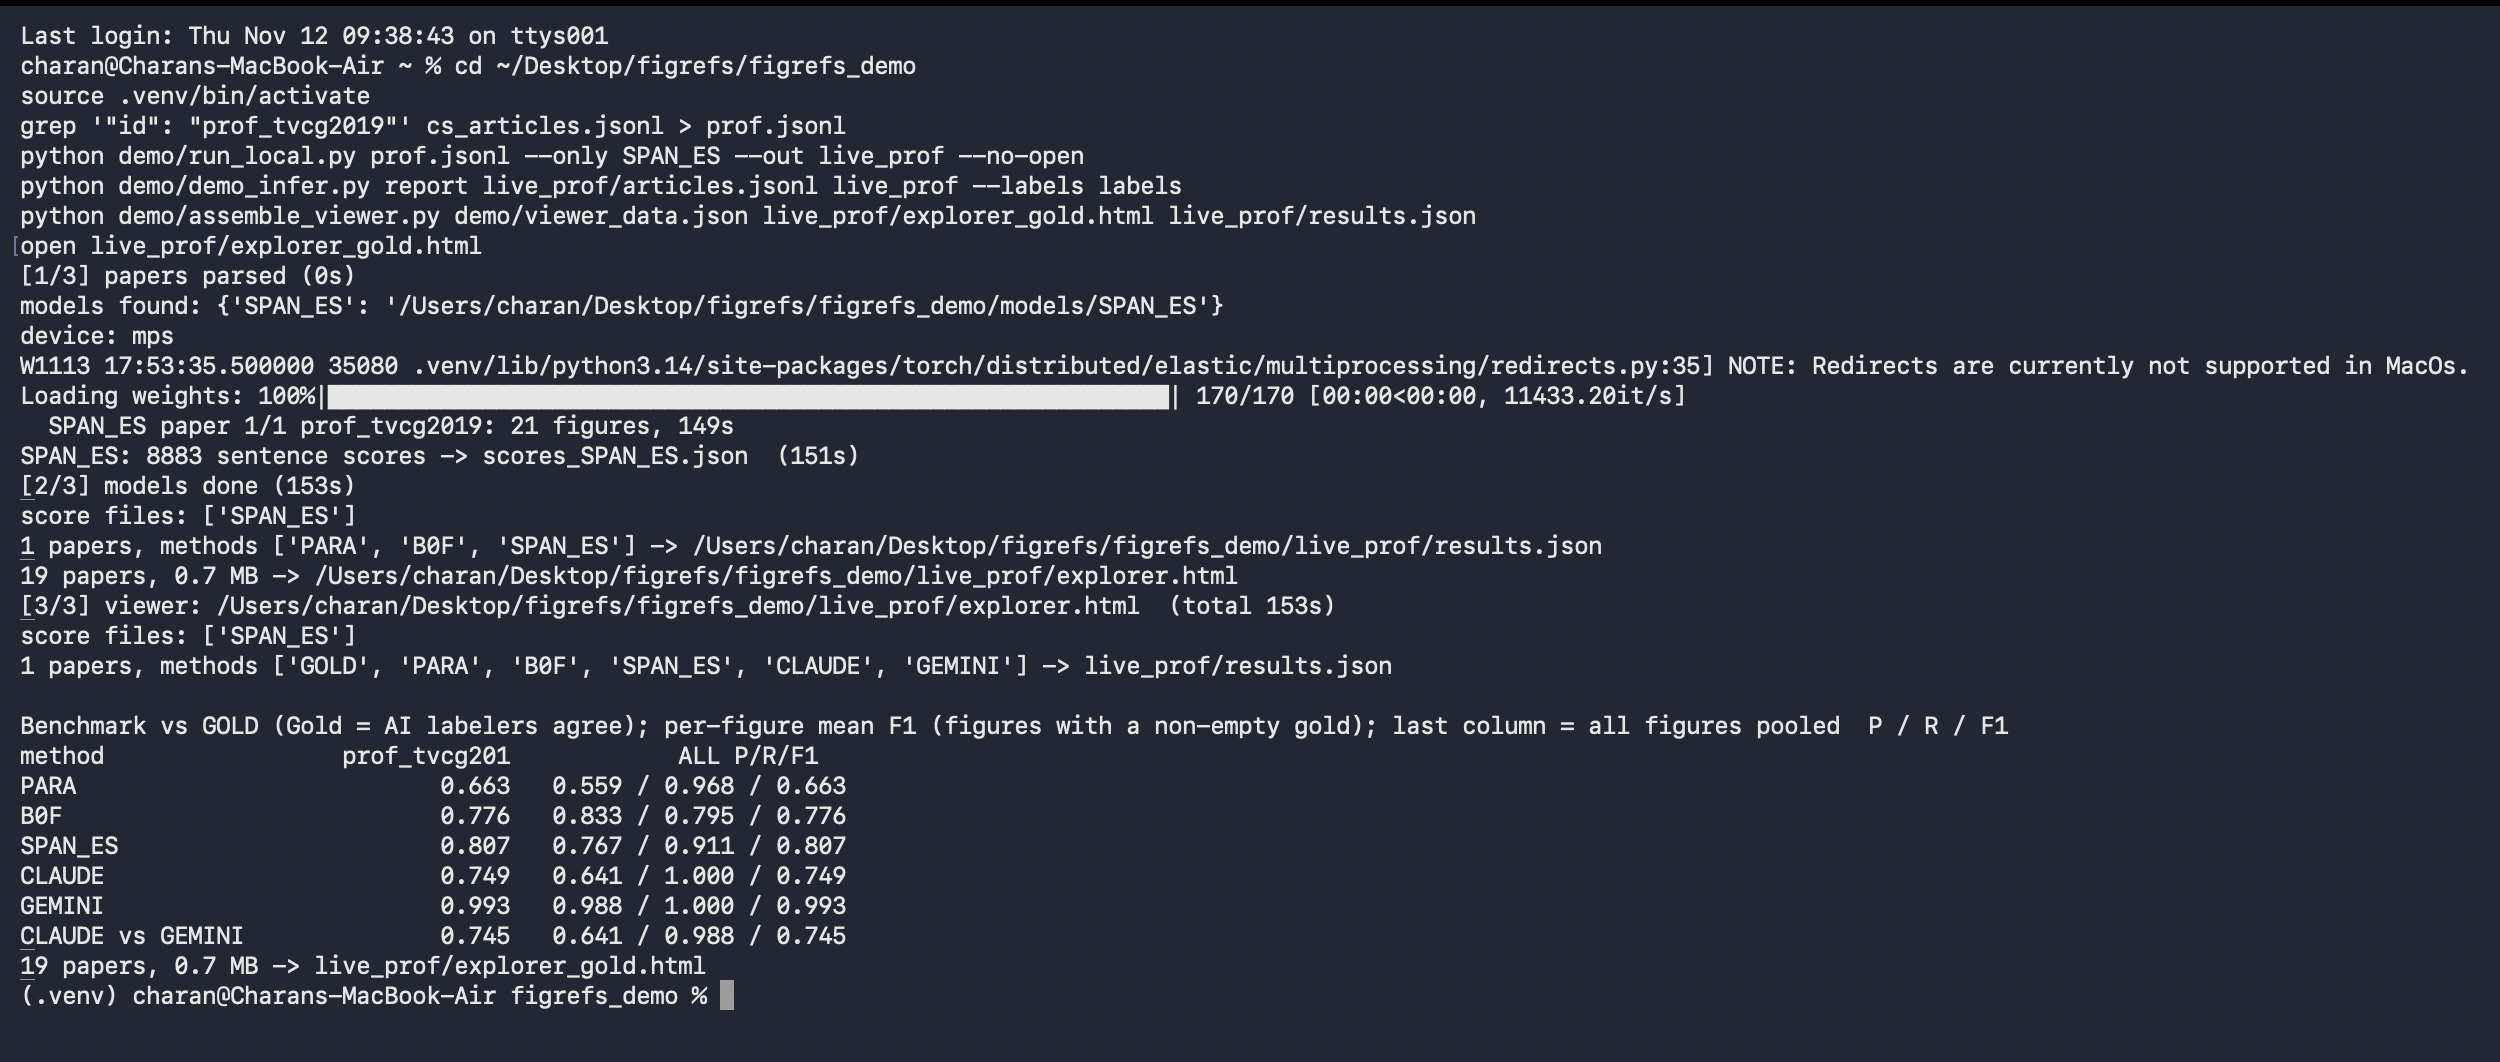
\includegraphics[width=\linewidth]{figures/cs_demo_run.png}
\caption{The inference script running SPAN\_ES on the computer-science paper on a laptop, followed by the
comparison with the LLM-agreement reference.}
\label{fig:cs}
\end{figure}

\begin{table}[h]
\centering
\small
\begin{tabular}{lrrr}
\toprule
System & P & R & F1\\
\midrule
Paragraph              & 0.559 & 0.968 & 0.663\\
\bof{} (rule)          & 0.833 & 0.795 & 0.776\\
\rowcolor{hl}
SPAN\_ES (our model)   & 0.767 & 0.911 & \best{0.807}\\
\midrule
\multicolumn{4}{l}{\emph{The two labellers themselves}}\\
Claude, against the agreement set   & 0.641 & 1.000 & 0.749\\
Gemini, against the agreement set   & 0.988 & 1.000 & 0.993\\
Claude against Gemini               & 0.641 & 0.988 & 0.745\\
\bottomrule
\end{tabular}
\caption{One computer-science paper (21 figures), scored against the sentences on which two LLM labellers
agree. This is a sanity check, not a benchmark; see the caveats in the text.}
\label{tab:cs}
\end{table}

\paragraph{What this shows.} The ordering found on biomedical papers is reproduced on a paper from a different
field: the model (0.807) is ahead of the rule (0.776), which is well ahead of Paragraph (0.663). As on
\figsum{}, the model's advantage is recall (0.911 against 0.795) at a moderate cost in precision. Neither the
rule nor the model was adjusted for this paper. We read this as evidence that what the model learned from 15
biomedical articles is not specific to biomedicine, and that the tool gives sensible output on
computer-science papers.

\paragraph{What this does not show.} We want to be explicit about how weak this evidence is as a measurement.
\begin{itemize}
  \item \textbf{The reference is not a gold standard.} It is the output of two language models that have not
        been validated for this task. On \figsum{}, where human labels exist, LLM annotators scored below our
        rule (Section~\ref{sec:othertrials}). The numbers in Table~\ref{tab:cs} measure agreement with those
        models, not correctness.
  \item \textbf{The two labellers disagree substantially.} Scored against each other they reach only 0.745,
        which is lower than the score of our model against their agreement set. A reference whose two sources
        agree at this level cannot support fine distinctions.
  \item \textbf{An agreement set favours the more conservative labeller.} Both labellers have a recall of
        1.0 against the reference, so the reference is in effect the intersection of their selections, and it
        is almost identical to the selection of the labeller that marks fewer sentences (Gemini, 0.993). The
        rows for the labellers are therefore not comparable with the rows for the systems, and the reference
        probably omits sentences that a human would include.
  \item \textbf{It is one paper.} Twenty-one figures from a single article are a very small sample.
  \item \textbf{Only the span tagger was run}, not the two-model ensemble of Section~\ref{sec:test}.
\end{itemize}
The language models were used here only to obtain a reference for evaluation. They are not part of the tool
and no model was trained on their labels. A proper out-of-domain evaluation needs human labels for
computer-science papers and is the first item of future work.
